%%
%% This is file `sample-sigchi.tex',
%% generated with the docstrip utility.
%% but modified by the faculty @ DI/FCUL
%% The original source files were:
%%
%% samples.dtx  (with options: `sigchi')
%% 
%% IMPORTANT NOTICE:
%% 
%% For the copyright see the source file.
%% 
%% Any modified versions of this file must be renamed
%% with new filenames distinct from sample-sigchi.tex.
%% 
%% For distribution of the original source see the terms
%% for copying and modification in the file samples.dtx.
%% 
%% This generated file may be distributed as long as the
%% original source files, as listed above, are part of the
%% same distribution. (The sources need not necessarily be
%% in the same archive or directory.)
%%
%% The first command in your LaTeX source must be the \documentclass command.
\documentclass[sigplan]{acmart}
\settopmatter{printacmref=false} % Removes citation information below abstract
\renewcommand\footnotetextcopyrightpermission[1]{} % removes footnote with conference information in first column
\usepackage{subcaption}
\usepackage{caption}
\usepackage{array}
\usepackage{multirow}
\usepackage{natbib}
\usepackage{graphicx}

%% end of the preamble, start of the body of the document source.
\begin{document}

\title{Title of Your Work}

\author{Afonso Carreira - 62701}
\affiliation{%
  \institution{
    Estudo Orientado \\
    Mestrado em Engenharia Informática \\
    Faculdade de Ciências, Universidade de Lisboa}
}
\email{fc62701@fc.ul.pt}


\begin{abstract}
  your abstract (about 10 lines).
\end{abstract}


%%
%% Keywords. The author(s) should pick words that accurately describe
%% the work being presented. Separate the keywords with commas.
\keywords{5 keywords}

\pagestyle{plain} % removes running headers

%%
%% This command processes the author and affiliation and title
%% information and builds the first part of the formatted document.
\maketitle
\section{Introduction}

This thesis aims to make programmers aware of the energy consumed by their programs. The time it takes to execute an algorithm and the memory it takes to perform a given task have always been issues that developers have been concerned about, and recently there have been attempts to reduce the energy cost of programs. However, building energy-efficient code is not a simple task and can often be overlooked. Because of its difficulty, there is still a need for tools that can help with this task\cite{10.1145/2597073.2597110}. 


Saving energy in programs is crucial for the operation of certain devices, such as mobile phones or IoT devices, so certain techniques need to be applied in order to reduce the energy of a program. For mobile devices, techniques are already used to save the battery when necessary, but for systems that don't use batteries, such as servers, energy is rarely taken into account when developing a program.
This lack of concern or awareness on the part of developers, although it appears to have a small impact, turns out to be quite significant, as in 2020 around 7\% of global electricity use is due to information and communications technology, with an anticipated rise in line with the growing demand for new technologies\cite{article}. This trend has become even more significant with the increased use of artificial intelligence \cite{patterson2021carbon}, especially large scale models such as ChatGPT, which require significant computing resources to train and run. These energy-intensive processes contribute significantly to global energy consumption and carbon emissions, raising environmental concerns as AI adoption continues to grow.

There are several reasons why there is a need to save energy in software, be it for mobile systems or data centers applications. \\

\begin{itemize}
  \item The dependence of mobile devices on batteries. All mobile devices rely on their batteries, so the software they run needs to make the best use of resources to conserve battery power.
  \item Reducing operating costs in data centers. It is crucial to reduce the operating cost of data centers by using energy-efficient programs. This reduction results in economic benefits for companies and contributes positively to environmental sustainability. 
  \item Reducing energy consumption has a benefic impact in our environment, as it saves energy that can be used for other things. \\
\end{itemize}

When, trying to improve the energy efficiency of their code, programmers rely on blogs, websites, YouTube videos and nowadays even chatbots like ChatGPT, which in most cases do not give completly right answers, and sometimes even the wrong ones. This is due to a lack of knowledge and guidelines.
Also, current tools can measure the energy of programs and applications as they run, but this usually requires extra steps that many developers may not have the time or inclination to take, so there is a need for a tool that can help the developer without the need for extra effort\cite{10.1145/3154384}. 

Many devices rely on Java and the Java Virtual Machine (JVM), so it is important that the code they run is energy efficient. Several factors can affect the power consumption of Java applications, including the behavior of the garbage collector and the efficiency of the memory management system \cite{10.5555/1267847.1267870} making it difficult to predict the power consumption of Java programs. This unpredictability highlights the need for a specialized tool to accurately measure and analyze power consumption so that developers can optimize their applications for energy efficiency.
Java is an excellent choice for developing this tool because of its high interoperability with various operating systems and its widespread usage across the globe, making it a reliable and option. It has a wide range of useful libraries (JRAPL, joularjx, Jalen) that help to measure energy accurately, and Java's typing and object-oriented features make the code easier to maintain and extend, so the tool can evolve with new energy metering standards and technologies. 

In order to create this tool, static analysis techniques will have to be used to understand which methods are going to be used and, through inferences from previously collected data, indicate the estimated energy levels of the program's execution. The inference will be made using energy data collected from low-level library functions. More complex functions are built on the basis of function composition, which means that, based on the estimated consumption of low-level functions, we can generalize our estimates to more complex functions and ultimately to the program as a whole. 

This work proposes the development of a solution capable of identifying the energy consumption of methods in programs and presenting this information quickly to the programmers, allowing them to make informed decisions in software design. The goal is to create an extension for an IDE that integrates these functionalities. This way, developers will have immediate feedback on the energy impact of their applications and can adjust them to meet efficiency requirements. Also the tool should be simple to use and developers should not need to know much about the energy to know how to use it. \\

\textbf{Organization} 

\begin{itemize}

\item Background (\ref{sec:background}) contains information of concepts that should be known to understand the complete report. It explains why it is difficult to predict and measure energy consumption of programs. It explains different energy tools, how they work, and what they do. It explains static and dynamic analysis and why it is important in this work.

\item Related work (\ref{sec:relatedwork}) contains the initials solutions proposed to the theme of energy aware programming, how they changed during the years, and what the most recent tools do. And comparing with the proposed tool in this work.

\item This section (\ref{sec:work1}) explains in detail the existing problem and what is the solution, and a detailed explaination on how the solution will be built.

\item The preliminary results (\ref{sec:preliminaryresults}) contains the tests made until the moment, and what results were obtained.

\item  Final conclusions (\ref{sec:conclusions}) of the work done until the moment, and explaination of what work will be continued to be done.\\
\end{itemize}


\section{Background} \label{sec:background}

To fully understand the processes involved in this work, it is important to first understand what energy profiling is, as it will be frequently referenced and used later.

Energy profiling is the systematic process of measuring, monitoring, and analyzing the power consumption of a system using specialized software or hardware tools to collect detailed power consumption data. This data can be collected from different parts of a system, including applications, processes, and specific snippets of code, to provide insight into how different components and activities contribute to overall energy consumption. Through this type of power consumption profiling, developers are able to identify inefficiencies and optimize software to improve energy efficiency. This makes it very important for extending battery life in mobile devices, reducing operating costs in data centers, and also minimizing environmental impact through energy consumption. Energy profiling is a step toward making informed decisions to develop more sustainable and cost-effective computing solutions.

When programming, developers usually consider the time it takes to complete a program, or the response time from client to server, or the amount of memory it uses. Most don't have an idea of how much energy their program consumes, or how much it can consume in certain cases, and getting this idea is not as trivial as it seems. To get this awareness, measurements could be made, but they are also difficult to get compared to measuring the time a program takes, which is checking the differences in timestamps, or understanding the memory usage. As for measuring energy, the same program can produce different values due to its non deterministic nature, meaning that results are often expressed as a range of possible values. Also, reducing the execution time of a program does not guarantee that the power consumption will follow. To obtain the measurements it is necessary to use some techniques that may require hardware devices for accurate values or software based tools that can facilitate this process, sometimes at the cost of less accurate readings.

To perform hardware-based measurements, a power monitor or power meter device must be used to obtain the precise values that a system uses when connected to the electrical grid. These devices measure the power drawn from the grid to the machine, but they usually measure the power consumed by the entire system rather than by specific pieces of hardware, which means they have low granularity.To gain this granularity and perform the measurements for only some parts of the machine, such as CPU and RAM, a harder setup is required to avoid reading unnecessary power consumption. This technique is not suitable for developers who only want to analyze the energy performance of their programs, which shows the difficulty of measuring energy consumption.

Another alternative is to use software-based tools. These tools are typically easier to use, but may not provide values as accurate as hardware-based measurements. However, they are more versatile and can be implemented or modified to meet the user's needs. 

\subsection{Energy Tools} \label{sec:background_energy}


There are some tools capable of displaying the energy consumption of programs.

Intel RAPL (Running Average Power Limit) is a tool for monitoring power consumption. It utilizes Model-Specific Registers (MSRs), which are used for program execution tracing, performance monitoring, and toggling CPU features. These registers can store the total energy usage of the CPU and memory, allowing it to be read and analyzed. Most software based tools rely on RAPL to measure energy consumption, since it is prety accurate and is widely available in most CPUs

Perf is a command line tool already available in linux, and is mainly used for performance monitoring and profiling. Although its not specific for energy measurement, it can do it, with Intel RAPL but not as pratical as other tools, specially when its needed to meausre a single process energy consumption.

Powertop is another tool capable of providing the power consumption, however it only works for laptops, as it requires to check the battery to see how much energy was used and calculate the power consumption.

Joularjx is a tool based on powerjoular and capable to measure energy consumption on Java programs, displaying the methods consumption.

Experiment-Runner is a framework built in python made to facilitate experiments, it is easily customizable and can be used with energy measurement tools to monitor the power consumption of another process.

To perform this work a tool is needed in order to measure the energy of programs, methods or code snippets. The tool used was powerjoular \cite{noureddine-ie-2022}, a open source tool, capable of measuring energy, from the CPU and GPU, using the Intel RAPL power data through the Linux powercap interface it can read the energy from the CPU and for the GPU it uses NVIDIA SMI to directly read the power consumption.
To read the power consumption of specific processes, PowerJoular monitors the CPU cycles and utilization of each process. By knowing the total power consumption of the CPU through the RAPL interface, it can calculate the power usage of individual processes based on their CPU utilization.
It is build in ADA, that is considered one of most energy efficient programming languages and it can monitor applications by name or PID.


\subsection{Code static and dynamic analysis} \label{sec:background_static_dynamic_analysis}
Also, the tool proposed in this work will mainly use static analysis to achieve its goal, so it is crucial to understand why it is preferred over dynamic analysis in this context.

Static analysis, as the name implies, analyzes the code statically, meaning it examines the code without executing it. By examining the code, static analysis tools can understand how the program will behave at runtime\cite{ernst2003static}, this analysis often aims for soundness, meaning that if the tool catches an error, it means that the error really exists, there are no false negatives. However, this can come at the cost of producing false positives, where issues that are not actually problems are flaged, so its important to keeps a balance between them. This analysis allows to check the entire source code and every path, much like compilers check syntax and types. Still, they can only predict some behaviors, as some can only be found when the program is executed, for example, by using dynamic analysis.

Dynamic analysis, on the other hand, executes the program and observes its exact behavior without having to estimate or predict. This type of analysis leaves no doubt about memory usage, output, the path taken, how much time it took\cite{ernst2003static}. A good example of dynamic analysis is unit testing, which tries to cover as many code paths as possible with different inputs, to understand as much as possible how the program works, and to find something that might be difficult to find with static analysis. However, dynamic analysis can be time consuming, especially for programs that take a long time to complete.

For fast power estimation, static analysis is preferable. It analyzes code faster and is better suited for large projects with multiple dependencies, where dynamic analysis can be very difficult to achieve due to complex setup and long execution times. Although static analysis may not be as accurate as dynamic analysis, it is still a viable solution. In addition, static analysis is more portable because its setup is much simpler than the more complex setup required for dynamic analysis.
Developers typically prefer not to run the program just to get an average measure of energy consumption for a code snippet or program, as it is time consuming and impractical. Therefore, using static analysis to infer energy consumption makes sense in this context.


\section{Related Work} \label{sec:relatedwork}

Energy efficiency is a critical focus across industries, as it directly impacts global sustainability, economic costs, and product quality.  The goal is to reduce greenhouse gases to create a sustainable future, reduce infrastructure costs, and improve product quality\cite{annurev:/content/journals/10.1146/annurev.resource.102308.124234}. 

In particular, large scale computation and communication consume a lot of global energy, and these values have been increasing in the last decades, so the topic of energy aware programming and energy efficient software has been targeted by many researchers in recent years with the objective of reducing energy costs in large IT infrastructure. This improvement can be considered a optimization problem and can be tackled in several ways for example an heuristic approach by adjusting the hardware performance dynamically, or completing tasks in their deadlines, using the least energy possible. However some of this implementations can only be short term solutions and in long term, the focus will be toward more complex models that can predict and optimize performance relative to hardware configurations\cite{10.1145/1666420.1666438}.

An approach to increasing developers awareness of the energy consumption of their code involves creating extensions to already used programming languages, such as Java. For example, ECO \cite{7194624}, a programming model as an minimal extension of Java. By rewriting some parts of the code to this extension syntax it is possible to defining resource limits on the battery or temperature implementing adaptive behaviors through modes, and leveraging runtime monitoring.

In addition, new languages can be developed to address these goals, as demonstrated by ENT\cite{10.1145/3062341.3062356}. ENT is a Java extension that empowers programmers with more direct control over the energy consumption of their applications. ENT’s type system enables applications to adapt dynamically to power constraints by switching operational modes based on resource availability, such as battery level or CPU temperature, allowing for software-level energy optimization. However, the language introduces complexity, making it potentially challenging for developers to learn and adapt to existing codebases. 

The use of static analysis can be valuable for understanding how instructions affect the energy consumption of programs. This paper\cite{aggarwal2014power} shows that system calls are directly related to energy consumption in Android applications. With this insight, it's possible to use static analysis to identify system calls within the code. This information can then be used to infer potential energy usage patterns, providing an early indication of where higher energy consumption may occur. This approach highlights the importance static analysis can have to understand program energy behaviors.

To tackle the problem of energy consumption in IT, some solutions have been presented. Some researchers focused on using energy measurement tools, like JRAPL to measure common libraries in Java and understand how much energy they use and what are the best alternatives to improve the energy efficiency of the code\cite{10.1145/2896967.2896968}. Observing common libraries for the implementation of list, sets and maps, is possible to see which ones have the better energy efficiency and what changes could improve the code.
Hasan et al.'s \cite{10.1145/2884781.2884869} research adds to this by creating detailed energy profiles for various Java collection classes, including lists, maps, and sets, across different implementations (Java Collections Framework, Apache Commons Collections, and Trove). Their work presents concrete quantification of energy consumption in these collections based on common operations such as insertion, iteration, and random access, and highlights the performance impact of collection types on energy efficiency for different input sizes.

However, because these collections are often used with threads, it is important to understand how much energy efficiency can be improved without compromising thread safety. The energy consumption of Java's thread-safe collections was studied in \cite{7816451}, where researchers demonstrated that switching to more energy-efficient collection implementations can reduce energy usage while maintaining thread safety.

Building on these efforts, \cite{10.1145/3238147.3240473}, Pereira et al. introduced a static analysis tool (Jstanley), as part of a Eclipse plugin, that can detect energy inefficient collections and recommend better alternatives. While jStanley demonstrated notable improvements in energy efficiency within its specific context, it has several limitations.
For example they only account for 3 collections, (Lists, Sets and Maps), they only account for 3 sizes of the collections (25,000, 250,000 and 1,000,000), it does not account for loops, thread safe and thread unsafe collections. Compared to our approach, Jstanley is limited, as it does not provide the actual information about the energy spent, it just shows recommendations. While the tool shows great improvements in its tested environment, replacing collections may not be enough in many practical cases. A more extensive tool, capable of analyzing a wider range of collections and providing energy metrics, would enable developers to achieve even greater energy efficiency and awareness.

In this work\cite{8816747}, a tool (CT+) has been proposed that is capable of performing static analysis of the code and recommending changes that reduce energy consumption. It improved from previous works by taking into account more collections implementations, more operations, thread safety and support for mobile applications. 

In addition, SEEP \cite{10.1145/2094091.2094106} uses symbolic execution for energy profiling, generating multiple binaries representing different code paths and input scenarios. By analyzing these binaries with hardware-based energy measurement devices, SEEP provides energy consumption data, offering a deeper understanding of code efficiency across various inputs and paths. This approach complements other tool, such as PEEK, which builds on SEEP to help developers optimize energy usage with minimal effort \cite{187026}. PEEK is an IDE-integrated framework that guides developers in writing energy-efficient code. It has a front end for IDE interfaces (e.g., Eclipse, Xcode), a middle end to manage data and versioning via Git, and a backend where energy analysis is performed—either through SEEP or hardware devices. Through these layers, PEEK identifies inefficiencies and suggests optimizations, supporting efficient coding practices. However, it has some limitations when compared to the proposed approach in this work, it uses dynamic analysis instead of static analysis, which was already explained in, \ref{sec:background_static_dynamic_analysis}, why it was choosen over dynamic analysis.


This solutions have some limitations, like the need to execute the code before showing the average energy cost to the developer and have limited collections.

This work has the objective of creating a user friendly tool that quickly estimates energy consumption through static analysis and providing developers recommendations. This energy will then be displayed to the developer making him more aware of the energy consumption of the program and help make better decisions.




%hasim collections
%oliveira Recommending Java Colletions (related work tem analise estatica)
%jsmeter
%analise estatica e dinamica
%Mario Linares-Vásquez (API de UI)
%Ivano Malavolta (API - Webassembler)
% 

Where the existing related technologies are described and explored. What is the state of the art on the topic you are working? 

\section{«Section(s) about your Work»} \label{sec:work1}

As described in the previous sections, the challenge is to make developers aware of the energy consumption of their programs. By using a simple and practical tool, they can quickly and accurately estimate their program's energy consumption. This allows them to get immediate feedback on energy consumption with every code change, facilitating energy-efficient development. It's important to note that this tool serves as a guide, providing energy consumption estimates to raise awareness rather than dictate action. Ultimately, it is up to developers to decide whether to prioritize performance, energy efficiency or any other factor. For example, if a program only needs to run within a certain timeframe and can afford a slight reduction in performance, developers may choose to trade some performance for improved energy efficiency, making more informed decisions thanks to the insights provided by the tool.

To provide this insight to developers it is necessary to build a tool that can provide all of that. The tool needs to be pratical, which means that integrating it in an IDE is a very good option. With this the developer only needs to download an extension for an IDE and will have the insights desired.
The tool will be an extension using Language Server Protocol (LSP), so it can be integrated in all the IDEs that support this feature (VScode, Eclipse, Neovim, Intellij IDEA). This will make it accessible to most developers wanting feedback on the energy consumption. To make it fast, it will use static analysis to parse the code into an Abstract Syntax Tree (ABS), from there its capable of analyzing the code and using an inference function it will output the estimated cost. \textbf{It will also be possible to make a more precise estimation, by running the code and also provide recommendations. optional/if i have time}.

-------------------------\\
The inference function will work like this \textbf{Understand how to do this}
First it is important to understand which snippets of code influence the energy consumption, what are the most common ones (sys calls/ CPU usage/ recursion/ loops ).
Maybe collect data from the powerjoular and use a ML model.
Maybe do it by hand with data analysis and obtain a formula capable of infering the energy.
-------------------------\\





Here you should describe in as much detail as possible the problem and your plan to tackle it (use appropriate section titles for the described work). \\

What are the methods you are planning to use, or already started to use, to tackle your problem. \\

This should be based on related word, your understanding of the problem and eventually preliminary results.

\section{Preliminary Results (optional)} \label{sec:preliminaryresults}

In the start of the project, some tools were tested in order to see how to get the energy profiles for later use. The tools tested were PowerJoular, powertop, perf and joularjx.

Perf is a Linux tool primarily designed for analyzing application performance characteristics rather than precise energy measurement. While it can provide some energy-related metrics, its measurements tend to be imprecise. In this context, perf was used mainly to get a rough idea of energy consumption and to serve as an alternative when more accurate tools were unavailable.

Powertop was also tested, but it could only perform energy measurements on laptops, as it relies on battery drain data to calculate energy consumption. Since this approach doesn't align with our specific requirements, we considered Powertop as a last-resort option.

Joularjx is a tool based on PowerJoular capable of measuring energy consumption of Java applications and it provides the energy used by the methods and overall program. Although it uses PowerJoular, when measuring the same program it gives different measurements.\textbf{why}

As described in the the \ref{sec:background_energy}, PowerJoular is the best option. As a command line program it can be easily adpated to measure any program or code snippet in most languages. So it was combined with the framework experiment-runner, that facilitates the process.


Initially, JoularJx and the experiment-runner using powerjoular were used to explore their capabilities and familiarize with the tools. A sample Fibonacci program written in Java and C was used as a test case. However, the energy measurements provided by the two tools differed, and the experiment runner occasionally encountered errors. Later, it was determined that these problems were due to incorrect use of the framework. However it was still decided the the best approach was to make a new orchestrator similar to the Experiment-Runner, but simpler and specifically focused on measuring process energy consumption using PowerJoular. A Java-based orchestrator was initially developed because the Fibonacci implementation was also in Java. However, when tested, the energy measurement results differed significantly from those of the experiment runner, even though the main difference was the programming language (Java vs. Python).

To further analyze these inconsistencies, another orchestrator was developed in Python. This allowed for a closer examination of the differences in energy measurements and a deeper understanding of the behavior of the tools.

To better understand the results and the problem encountered, its better to see, first, how the orchestrators behave:


\begin{itemize}
  \item On the start of the orchestrator it launches a command to start the target Java Program and waits a signal.
  \item The Java program start and setup the necessary things to run (starting threads, reading/writing files, etc.) and then it sends a start signal to the orchestrator to start monitoring the computation wanted, and waits for some miliseconds. 
  \item The orchestrator receives the start signal and reads the PID of the target program from a file and starts PowerJoular using that PID. Then it waits for the stop signal.
  \item The target Java program when it finishes the computation it sends a stop signal back.
  \item The orchestrator on receiving the stop signal, first stops PowerJoular and then stops the target program, if needed. Then it displays the energy measurement information stored in the files created by PowerJoular. \\
\end{itemize}

This process is more clearly illustrated in Figure \ref{fig:orchestrators_process}

\begin{figure}%[h]
  \centering
  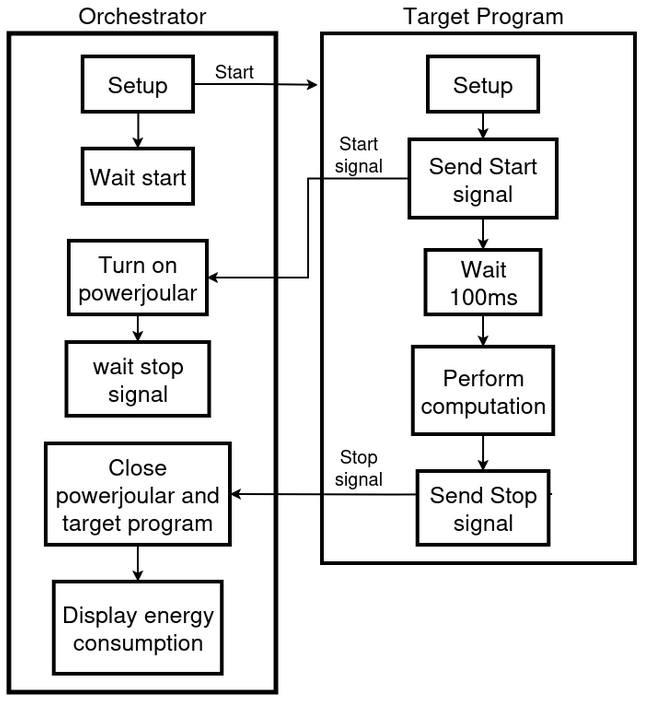
\includegraphics[width = 0.4 \textwidth]{figures/orchestrators_process.png}
  \caption{orchestrators process}
  \label{fig:orchestrators_process}
\end{figure}

With this process it was noticeble that the Java orchestrator was getting significantly more energy consumption than the Python one, which is not very logical, since they both target the same program. So, to try and check which one was having problems, two more orchestrators were implemented, one in C and another in bash.

After running the tests again it was possible to see that the Python orchestrator was getting values way more different than the other three orchestrators as show in Figure \ref{fig:4_orchs_comparison}.
The figure contains 100 runs of the Fibonacci recursive program written in Java and order by the less energy to highest energy. And it shows the energy reads for the four different orchestrators used. The labels contain the average energy values and its standard deviation.

Further analysis of the orchestrators revealed a notable difference in behavior. When the Python orchestrator was running, both the parent and child processes consumed CPU resources. In contrast, the other orchestrators (Java, C, and Bash) showed CPU usage only in the child process. This disparity may explain why powerjoular reported lower energy consumption for the Python orchestrator. Since the CPU load was shared between the parent and child processes, powerjoular, which measures energy only for the child process (the target Fibonacci program), captured less total energy usage.
Since the experiment runner included an example demonstrating how to use the framework with powerjoular, the authors were made aware of this potential conflict when launching powerjoular from Python.

\begin{figure}%[h]
  \centering
  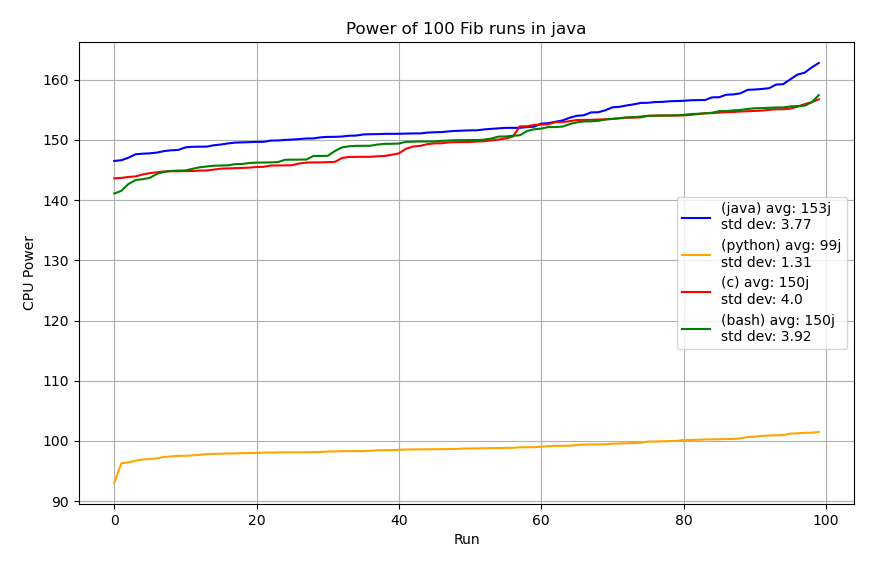
\includegraphics[width = 0.5 \textwidth]{figures/4_orchestrators_comparison.png}
  \caption{orchestrators comparison}
  \label{fig:4_orchs_comparison}
\end{figure}

\section{Forthcoming Work and Conclusions} \label{sec:conclusions}

Possible work timeline

\begin{figure}[h]
  \centering
  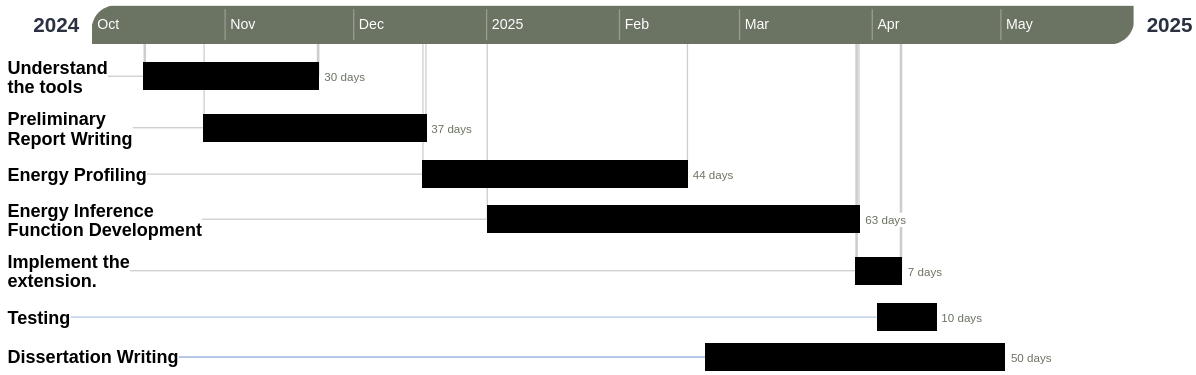
\includegraphics[width = 0.5 \textwidth]{figures/gantt_diagram.png}
  \caption{Work}
  \label{fig:gantt_diagram}
\end{figure}


It should include subsections that describe the work to be carried out during the rest of the year, and what its objectives are.

It should also include planning until the end of the work, in chronological order.

Include a final concluding subsection (may be a separate section) with a summary of contributions already made, a preliminary self-assessment of the work done so far, and difficulties encountered.


%%%%%%%%%%%%%%%%%%%%%%%%%%%%%%%%%%%%%%%%%%%%%%%%%%%%%%%%%%%%%%%%%%%%%%
%% The next two lines define the bibliography style to be used, and
%% the bibliography file.
\bibliographystyle{unsrt}
\bibliography{ref}
\end{document}
